\chapter{Advanced Topics}

\index{inheritance}
\index{generalization}

When we first looked at inheritance in Chapter~\ref{eights}, our purpose was to avoid duplicating code.
We noticed that ``decks of cards'' and ``hands of cards'' had common functionality, and we designed a \java{CardCollection} class to provide it.
This technique is an example of {\bf generalization}.
By generalizing the code, we were able to reuse it in the \java{Deck} and \java{Hand} classes.

\index{specialization}

In Chapter~\ref{conway}, we looked at inheritance from a different point of view.
When designing \java{GridCanvas} to represent a grid of cells, we extended \java{Canvas} and overrode its \java{paint} method.
This design is an example of {\bf specialization}.
Using the code provided by \java{Canvas}, we created a specialized subclass with minimal additional code.

We didn't write the code for \java{Canvas}; it's part of the Java Library.
But we were able to customize it for our own purposes.
In fact, the \java{Canvas} class was explicitly designed to be extended.

In this chapter, we'll explore the concept of inheritance more fully and explore event-driven programming.
We'll continue to develop graphical simulations as a running example, but this time in varying shapes and colors!


\section{Polygon Objects}

The word polygon means ``many angles''; the most basic polygons are triangles (3 angles), rectangles (4 angles), pentagons (5 angles), and so forth.
Polygons are an important part of computer graphics because they are used to compose more complex images.

Java provides a \java{Polygon} class (in \java{java.awt}) that we can use to represent and draw polygons.
The following code creates an empty \java{Polygon} and adds three points, forming a triangle.

\begin{code}
Polygon p = new Polygon();
p.addPoint(57, 110);
p.addPoint(100, 35);
p.addPoint(143, 110);
\end{code}

Internally, \java{Polygon} objects have three attributes:

\begin{itemize}

\item \java{public int npoints;} {\tt ~~~} \java{// total number of points}

\item \java{public int[] xpoints;} {\tt ~} \java{// array of X coordinates}

\item \java{public int[] ypoints;} {\tt ~} \java{// array of Y coordinates}

\end{itemize}

When a \java{Polygon} is created, \java{npoints} is 0 and the two arrays are initialized with length 4.
As points are added, \java{npoints} is incremented.
If \java{npoints} exceeds the length of the arrays, larger arrays are created, and the previous values are copied over (similar to how \java{ArrayList} works).

The \java{Polygon} class provides many useful methods, like \java{contains}, \java{intersects}, and \java{translate}.
We'll get to those later, but first we're going to do some specialization.


\section{Adding Color}

Specialization is useful for adding new features to an existing class, especially when you can't (or don't want to) change its design.
For example, we can extend the \java{Polygon} class by adding a \java{draw} method and a \java{Color} attribute:

\begin{code}
public class DrawablePolygon extends Polygon {
    public Color color;

    public DrawablePolygon() {
        super();
        color = Color.GRAY;
    }

    public void draw(Graphics g) {
        g.setColor(color);
        g.fillPolygon(this);
    }
}
\end{code}

As a reminder, constructors are not inherited when you extend a class.
If you don't define a constructor, the compiler will generate one that does nothing.

The constructor for \java{DrawablePolygon} uses \java{super} to invoke the constructor for \java{Polygon}, which initializes the attributes \java{npoints}, \java{xpoints}, and \java{ypoints}.
Then \java{DrawablePolygon} initializes the \java{color} attribute to \java{GRAY}.

\java{DrawablePolygon} has the same attributes and methods that \java{Polygon} has, so you can use \java{addPoint} as before, or you can directly access \java{npoints}, \java{xpoints}, and \java{ypoints} (since they are \java{public}).
You can also use methods like \java{contains}, \java{intersects}, and \java{translate}.

The following code creates a \java{DrawablePolygon} with the same points as in the previous section and sets its color to \java{GREEN}:

\begin{code}
DrawablePolygon p = new DrawablePolygon();
p.addPoint(57, 110);
p.addPoint(100, 35);
p.addPoint(143, 110);
p.color = Color.GREEN;
\end{code}


\section{Regular Polygons}

A ``regular'' polygon has all sides the same length and all angles equal in measure.
Regular polygons are a special case of polygons, so we will use specialization to define a class for them.

We could extend the \java{Polygon} class, like we did in the previous section.
But then we would not have the \java{Color} functionality we just added.
So we will make \java{RegularPolygon} extend \java{DrawablePolygon}.

To construct a \java{RegularPolygon}, we specify the number of sides, the radius (distance from the center to a vertex), and the color.
For example:

\begin{code}
RegularPolygon rp = new RegularPolygon(6, 50, Color.BLUE);
\end{code}

\begin{figure}[!ht]
\begin{center}
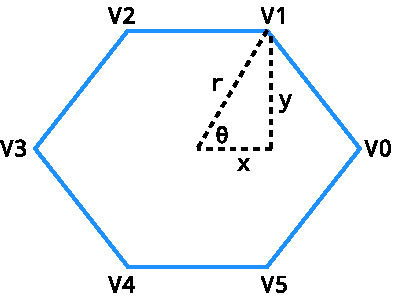
\includegraphics{figs/hexagon.pdf}
\caption{Determining the $x$ and $y$ coordinates of vertex V1, given the radius~$r$ and angle~$\theta$.
The center of the polygon is at the origin $(0, 0)$.}
\label{fig:hexagon}
\end{center}
\end{figure}

The constructor uses trigonometry to find the coordinates of each vertex.
Figure~\ref{fig:hexagon} illustrates the process.
The number of sides ($n=6$) and the radius ($r=50$) are given as parameters.

\begin{itemize}

\item Imagine a clock hand starting at V0 and rotating counterclockwise to V1, V2, and so forth.
In Figure~\ref{fig:hexagon}, the hand is currently at V1.

\item The angle $\theta$ is $2 \pi / n$, since there are $2\pi$ radians in a circle.
In other words, we are dividing the rotation of the clock hand into $n$ equal angles.

\item By definition, $\cos(\theta) = x/r$ and $\sin(\theta) = y/r$.
Therefore, $x = r \cos(\theta)$ and $y = r \sin(\theta)$.

\item We can determine the other $(x, y)$ coordinates by multiplying $\theta$ by $i$, where $i$ is the vertex number.

\end{itemize}

Here is the constructor for \java{RegularPolygon}:

\begin{code}
public RegularPolygon(int nsides, int radius, Color color) {

    // initialize DrawablePolygon attributes
    this.npoints = nsides;
    this.xpoints = new int[nsides];
    this.ypoints = new int[nsides];
    this.color = color;

    // the amount to rotate for each vertex (in radians)
    double theta = 2.0 * Math.PI / nsides;

    // compute x and y coordinates, centered at the origin
    for (int i = 0; i < nsides; i++) {
        double x = radius * Math.cos(i * theta);
        double y = radius * Math.sin(i * theta);
        xpoints[i] = (int) Math.round(x);
        ypoints[i] = (int) Math.round(y);
    }
}
\end{code}

This constructor initializes all four \java{DrawablePolygon} attributes, so it doesn't have to invoke \java{super()}.

It initializes \java{xpoints} and \java{ypoints} by creating arrays of integer coordinates.
Inside the \java{for} loop, it uses \java{Math.sin} and \java{Math.cos} (see Section~\ref{mathmeth}) to compute the coordinates of the vertices as floating-point numbers.
Then it rounds them off to integers, and stores them in the arrays.

When we construct a \java{RegularPolygon}, the vertices are centered at the point $(0, 0)$.
If we want the center of the polygon to be somewhere else, we can use \java{translate}, which we inherit from \java{Polygon}:

\begin{code}
RegularPolygon rp = new RegularPolygon(6, 50, Color.BLUE);
rp.translate(100, 100);
\end{code}

The result is a 6-sided polygon with radius 50 centered at the point $(100, 100)$.

% TODO suggestion from Marc Loy:
% Maybe a screenshot of a this exact polygon on a 200x200 canvas
% with some callouts on the center coordinate and radius to V0?


\section{More Constructors}

Classes in the Java library often have more than one constructor for convenience.
We can do the same with \java{RegularPolygon}.
For example, we can make the \java{color} parameter optional by defining a second constructor:

\begin{code}
public RegularPolygon(int nsides, int radius) {
    this(nsides, radius, Color.GRAY);
}
\end{code}

The keyword \java{this}, when used in a constructor, invokes another constructor in the same class.
It has a similar syntax as the keyword \java{super}, which invokes a constructor in the superclass.

Similarly, we could make the \java{radius} parameter optional too:

\begin{code}
public RegularPolygon(int nsides) {
    this(nsides, 50);
}
\end{code}

Now, suppose we invoke the \java{RegularPolygon} constructor like this:

\begin{code}
RegularPolygon rp = new RegularPolygon(6);
\end{code}

Because we provide only one integer argument, Java calls the third constructor, which calls the second one, which calls the first one.
The result is a \java{RegularPolygon} with the specified value of \java{nsides}, 6, the default value of \java{radius}, 50, and the default color, \java{GRAY}.

When writing constructors, it's a good idea to validate the values you get as arguments.
Doing so prevents run-time errors later in the program, which makes the code easier to debug.

For \java{RegularPolygon}, the number of sides should be at least three, the radius should be greater than zero, and the color should not be \java{null}.
We can add the following lines to the first constructor:

\begin{code}
public RegularPolygon(int nsides, int radius, Color color) {

    // validate the arguments
    if (nsides < 3) {
        throw new IllegalArgumentException("invalid nsides");
    }
    if (radius <= 0) {
        throw new IllegalArgumentException("invalid radius");
    }
    if (color == null) {
        throw new NullPointerException("invalid color");
    }

    // the rest of the method is omitted
\end{code}

\index{throw}
\index{Statement!throw}

In this example, we \java{throw} an exception to indicate that one of the arguments is invalid.
By default, these exceptions terminate the program and display an error message along with the stack trace.

Because we added this code to the most general constructor, we don't have to add it to the others.


\section{An Initial Drawing}
\label{sec:drawing}

Now that we have \java{DrawablePolygon} and \java{RegularPolygon}, let's take them for a test drive.
We'll need a \java{Canvas} for drawing them, so we define a new class, \java{Drawing}, that extends \java{Canvas}:

\begin{code}
public class Drawing extends Canvas {
    private ArrayList<DrawablePolygon> list;

    public Drawing(int width, int height) {
        setSize(width, height);
        setBackground(Color.WHITE);
        list = new ArrayList<DrawablePolygon>();
    }
\end{code}

\begin{code}
    public void add(DrawablePolygon cp) {
        list.add(cp);
    }

    public void paint(Graphics g) {
        for (DrawablePolygon dp : list) {
            dp.draw(g);
        }
    }
}
\end{code}

The \java{Drawing} class has an \java{ArrayList} of \java{DrawablePolygon} objects.
When we create a \java{Drawing} object, the list is initially empty.
The \java{add} method takes a \java{DrawablePolygon} and adds it to the list.

\java{Drawing} overrides the \java{paint} method that it inherits from \java{Canvas}.
\java{paint} loops through the list of \java{DrawablePolygon} objects and invokes \java{draw} on each one.

Here is an example that creates three \java{RegularPolygon} objects and draws them.
Figure~\ref{fig:drawing} shows the result.

\begin{code}
public static void main(String[] args) {

    // create some regular polygons
    DrawablePolygon p1 = new RegularPolygon(3, 50, Color.GREEN);
    DrawablePolygon p2 = new RegularPolygon(6, 50, Color.ORANGE);
    DrawablePolygon p3 = new RegularPolygon(360, 50, Color.BLUE);

    // move them out of the corner
    p1.translate(100, 80);
    p2.translate(250, 120);
    p3.translate(400, 160);

    // create drawing, add polygons
    Drawing drawing = new Drawing(500, 250);
    drawing.add(p1);
    drawing.add(p2);
    drawing.add(p3);
\end{code}

\begin{code}
    // set up the window frame
    JFrame frame = new JFrame("Drawing");
    frame.setDefaultCloseOperation(JFrame.EXIT_ON_CLOSE);
    frame.add(drawing);
    frame.pack();
    frame.setVisible(true);
}
\end{code}

\begin{figure}[!ht]
\begin{center}
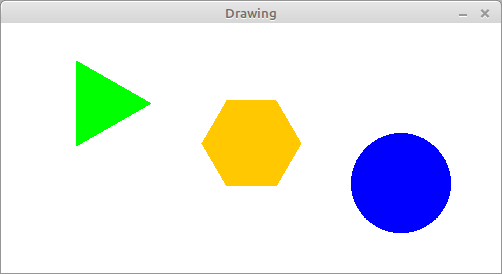
\includegraphics[width=4in]{figs/drawing.png}
\caption{Initial drawing of three \java{RegularPolygon} objects.}
\label{fig:drawing}
\end{center}
\end{figure}

The first block of code creates \java{RegularPolygon} objects with 3, 6, and 360 sides.
As you can see, a polygon with 360 sides is a pretty good approximation of a circle.

The second block of code translates the polygons to different locations.
The third block of code creates the \java{Drawing} and adds the polygons to it.
And the fourth block of code creates a \java{JFrame}, adds the \java{Drawing} to it, and displays the result.

Most of these pieces should be familiar, but there is one part of this program that might surprise you.
When we create the \java{RegularPolygon} objects, we assign them to \java{DrawablePolygon} variables.
%, and then pass them to \java{Drawing.add}, which requires \java{DrawablePolygon} objects.
It might not be obvious why that's legal.

\index{IS-A}

\java{RegularPolygon} extends \java{DrawablePolygon}, so every \java{RegularPolygon} object is also a \java{DrawablePolygon}.
The parameter of \java{Drawing.add} has to be a \java{DrawablePolygon}, but it can be any type of \java{DrawablePolygon}, including \java{RegularPolygon} and other subclasses.

\index{polymorphism}

This design is an example of {\bf polymorphism}, a fancy word that means ``having many forms''.
\java{Drawing.add} is polymorphic method, because the parameter can be one of many types.
And the \java{ArrayList} in \java{Drawing} is a polymorphic data structure, because the elements can be different types.

%At compile-time, \java{p1} is treated like a \java{DrawablePolygon}.
%But at run-time, \java{p1} is actually a \java{RegularPolygon}.

%What's interesting about this example is that the polygon objects have methods from multiple classes.
%The constructor is defined in \java{RegularPolygon}.
%The \java{translate} method is defined in \java{Polygon}.
%The \java{draw} method (called by \java{paint}) is defined in \java{DrawablePolygon}.
%And yet, everything works together seamlessly.


\section{Blinking Polygons}

At this point, we have a simple program that draws polygons; we can make it more fun by adding animation.
Chapter~\ref{conway} introduced the idea of simulating time steps.
Here's a loop that runs the animation.

\begin{code}
while (true) {
    drawing.step();
    try {
        Thread.sleep(1000 / 30);
    } catch (InterruptedException e) {
        // do nothing
    }
}
\end{code}

Each time through the loop, we call \java{step} to update the \java{Drawing}.
Then we sleep with a delay calculated to update about 30 times per second.

Here's what the \java{step} method of \java{Drawing} looks like:

\begin{code}
public void step() {
    for (DrawablePolygon dp : list) {
        dp.step();
    }
    repaint();
}
\end{code}

It invokes \java{step} on each \java{DrawablePolygon} in the list and then repaints (clears and redraws) the canvas.

In order for this code to compile, we need \java{DrawablePolygon} to provide a \java{step} method.
Here's a version that doesn't do anything; we'll override it in subclasses.

\begin{code}
public void step() {
    // do nothing
}
\end{code}

Now let's design a new type of polygon that blinks.
We'll define a class named \java{BlinkingPolygon} that extends \java{RegularPolygon} and adds two more attributes: \java{visible}, which indicates whether the polygon is visible, and \java{count}, which counts the number of time steps since the last blink.

\begin{code}
public class BlinkingPolygon extends RegularPolygon {
    public boolean visible;
    public int count;

    public BlinkingPolygon(int nsides, int radius, Color c) {
        super(nsides, radius, c);
        visible = true;
        count = 0;
    }

    public void draw(Graphics g) {
        if (visible) {
            super.draw(g);
        }
    }

    public void step() {
        count++;
        if (count == 10) {
            visible = !visible;
            count = 0;
        }
    }
}
\end{code}

The constructor uses \java{super} to call the \java{RegularPolygon} constructor.
Then it initializes \java{visible} and \java{count}.
Initially the \java{BlinkingPolygon} is visible.

The \java{draw} method draws the polygon only if it is visible.
It uses \java{super} to call \java{draw} in the parent class.
But the parent class is \java{RegularPolygon}, which does not provide a \java{draw} method.
In this case, \java{super} invokes \java{draw} from the \java{DrawablePolygon} class.

The \java{step} method increments \java{count}.
Every 10 time steps, it toggles \java{visible} and resets \java{count} to 0.


\section{Interfaces}

You might be getting tired of polygons at this point.
Can't we draw anything else?
Of course we can, but \java{Drawing} is currently based on \java{DrawablePolygon}.
To draw other types of objects, we have to generalize the code.

The \java{Drawing} class does essentially three things: (1) it maintains a \java{list} of objects, (2) it invokes the \java{draw} method on each object, and (3) it invokes the \java{step} method on each object.

So here's one way we could make the code more general:

\begin{enumerate}

\item Define a new superclass, which we call \java{Actor}, that provides the two methods needed by \java{Drawing}:

\begin{code}
public class Actor {
    public void draw(Graphics g) {
        // do nothing
    }
    public void step() {
        // do nothing
    }
}
\end{code}

\item In the \java{Drawing} class, replace \java{DrawablePolygon} with \java{Actor}.

\item Any class that we want to draw must now extend \java{Actor}.

\end{enumerate}

There's just one problem: \java{DrawablePolygon} already extends \java{Polygon}, and classes can only extend one superclass.
Also, the \java{Actor} class seems pointless, since the methods it defines don't do anything.

\index{inheritance}

Java provides another mechanism for inheritance that solves these problems.
We can define \java{Actor} as an \java{interface} instead of a \java{class}, like this:

\begin{code}
public interface Actor {
    void draw(Graphics g);
    void step();
}
\end{code}

\index{interface}

Like a class definition, an {\bf interface} definition contains methods.
But it contains only the declarations of the methods, not their implementations.

Like an abstract class, an interface specifies methods that must be provided by subclasses.
The difference is that an abstract class can implement some methods; an interface cannot.

All interface methods are \java{public} by default, since they are intended to be used by other classes.
So there is no need to declare them as \java{public}.

To inherit from an interface, you use the keyword \java{implements} instead of \java{extends}.
Here's a version of \java{DrawablePolygon} that extends \java{Polygon} and implements \java{Actor}.
So it inherits methods from \java{Polygon}, and it is required to provide the methods in \java{Actor}, namely \java{step} and \java{draw}.

\begin{code}
public class DrawablePolygon extends Polygon implements Actor {
    // rest of the class omitted
}
\end{code}

In terms of inheritance, \java{DrawablePolygon} is both a \java{Polygon} and an \java{Actor}.
So the following assignments are legal:

\begin{code}
Polygon p1 = new DrawablePolygon();
Actor a2 = new DrawablePolygon();
\end{code}

And the same is true for subclasses of \java{DrawablePolygon}; these assignments are legal, too:

\begin{code}
Polygon p2 = new RegularPolygon(5, 50, Color.YELLOW);
Actor a2 = new RegularPolygon(5, 50, Color.YELLOW);
\end{code}

\index{polymorphism}

Interfaces are another example of polymorphism.
\java{a1} and \java{a2} are the same type of variable, but they refer to objects with different types.
And similarly with \java{p1} and \java{p2}.

% But each of them provides the \java{draw} and \java{step} methods specified in the \java{Actor} interface.

Classes may extend only one superclass, but they may implement as many interfaces as needed.
Java Library classes often implement multiple interfaces.


\section{Event Listeners}

\index{sprite}

Now that our \java{Drawing} is based on \java{Actor} instead of \java{DrawablePolygon}, we can draw other types of graphics.
Here is the beginning of a class that reads an image from a file and shows the image moving across the canvas.
The class is called \java{Sprite} because a moving image is sometimes called a {\bf sprite}, in the context of computer graphics.

\begin{code}
public class Sprite implements Actor, KeyListener {
    private int xpos;
    private int ypos;
    private int dx;
    private int dy;
    private Image image;

    public Sprite(String path, int xpos, int ypos) {
        this.xpos = xpos;
        this.ypos = ypos;
        try {
            this.image = ImageIO.read(new File(path));
        } catch (IOException exc) {
            exc.printStackTrace();
        }
    }
}
\end{code}

The instance variables \java{xpos} and \java{ypos} represent the location of the sprite.
\java{dx} and \java{dy} represent the velocity of the sprite in the $x$ and $y$ directions.

The constructor takes as parameters the name of a file and the initial position.
It uses  \java{ImageIO}, from the \java{javax.imageio} package, to read the file.
If an error occurs during reading, an \java{IOException} is caught, and the program displays the stack trace for debugging.

\java{Sprite} implements two interfaces: \java{Actor} and \java{KeyListener}.
\java{Actor} requires that we provide \java{draw} and \java{step} methods:

\begin{code}
    public void draw(Graphics g) {
        g.drawImage(image, xpos, ypos, null);
    }

    public void step() {
        xpos += dx;
        ypos += dy;
    }
\end{code}

The \java{draw} method draws the image at the sprite's current position.
The \java{step} method changes the position based on \java{dx} and \java{dy}, which are initially zero.

\java{KeyListener} is an interface for receiving keyboard events, which means we can detect and respond to key presses.
A class that implements \java{KeyListener} has to provide the following methods:

\begin{itemize}

\item \java{void keyPressed(KeyEvent e);}
\\ Invoked when a key has been ``pressed''.
This method is invoked repeatedly while a key is being held down.

\item \java{void keyReleased(KeyEvent e);}
\\ Invoked when a key has been ``released'', meaning it is no longer down.

\item \java{void keyTyped(KeyEvent e);}
\\ Invoked when a key has been ``typed'', which generally means it has been both pressed and released.

\end{itemize}

These methods get invoked when the user presses and releases {\em any} key.
They take a \java{KeyEvent} object as a parameter, which specifies which key was pressed, released, or typed.

We can use these methods to design a simple animation using the arrow keys.
When the user presses up or down, the sprite will move up or down.
When the user presses left or right, the sprite will move left or right.

Here's an implementation of \java{keyPressed} that uses a \java{switch} statement to test which arrow key was pressed and sets \java{dx} or \java{dy} accordingly.
(There is no \java{default} branch, so we ignore all other keys.)

\begin{code}
public void keyPressed(KeyEvent e) {
    switch (e.getKeyCode()) {
        case KeyEvent.VK_UP:
            dy = -5;
            break;
        case KeyEvent.VK_DOWN:
            dy = +5;
            break;
        case KeyEvent.VK_LEFT:
            dx = -5;
            break;
        case KeyEvent.VK_RIGHT:
            dx = +5;
            break;
    }
}
\end{code}

The values of \java{dx} and \java{dy} determine how much the sprite moves each time \java{step} is invoked.
While the user holds down an arrow key, the sprite will move at a constant speed.

Here's an implementation of \java{keyReleased} that runs when the user releases the key.

\begin{code}
public void keyReleased(KeyEvent e) {
    switch (e.getKeyCode()) {
        case KeyEvent.VK_UP:
        case KeyEvent.VK_DOWN:
            dy = 0;
            break;
        case KeyEvent.VK_LEFT:
        case KeyEvent.VK_RIGHT:
            dx = 0;
            break;
    }
}
\end{code}

When the user releases the key, \java{keyReleased} sets \java{dx} or \java{dy} to 0, so the sprite stops moving in that direction.

We don't need the \java{keyTyped} method for this example, but it's required by the interface; if we don't provide one, the compiler will complain.
So we provide an implementation that does nothing:

\begin{code}
public void keyTyped(KeyEvent e) {
    // do nothing
}
\end{code}

Now, here's the code we need to create a \java{Sprite}, add it to a \java{Drawing}, and configure it as a \java{KeyListener}:

\begin{code}
Sprite sprite = new Sprite("face-smile.png", 25, 150);
drawing.add(sprite);
drawing.addKeyListener(sprite);
drawing.setFocusable(true);
\end{code}

Recall that the \java{add} method is one that we wrote in Section~\ref{sec:drawing}.
It adds an \java{Actor} to the list of objects to be drawn.

The \java{addKeyListener} method is inherited from \java{Canvas}.
It adds a \java{KeyListener} to the list of objects that will receive key events.

In graphical applications, key events are only sent to components when they have the keyboard focus.
The \java{setFocusable} method ensures that \java{drawing} will be have the focus initially, without the user having to click on it first.


\section{Timers}

%When you run this program, the arrow keys might not work initially.
%If that happens, click on the drawing to give it the keyboard focus.

Now that you know about interfaces and events, we can show you a better way to create animations.
Previously, we implemented the animation loop using \java{while (true)} and \java{Thread.sleep}.
Java provides a \java{Timer} class (in \java{javax.swing}) that encapsulates this behavior.

A \java{Timer} is useful for executing code at regular intervals.
The constructor for \java{Timer} takes two parameters:

\begin{itemize}
\item \java{int delay} {\tt ~~~~~~~~~~~~~~~} \java{// milliseconds between events}

\item \java{ActionListener listener} {\tt ~} \java{// for handling timer events}
\end{itemize}

The \java{ActionListener} interface requires only one method, \java{actionPerformed}.
This is the method the \java{Timer} invokes after the given delay.

Using a \java{Timer}, we can reorganize the code in \java{main} by defining a class that implements \java{ActionListener}.

\begin{code}
public class VideoGame implements ActionListener {
    private Drawing drawing;

    public VideoGame() {
        Sprite sprite = new Sprite("face-smile.png", 50, 50);
        drawing = new Drawing(800, 600);
        drawing.add(sprite);
        drawing.addKeyListener(sprite);
        drawing.setFocusable(true);

        JFrame frame = new JFrame("Video Game");
        frame.setDefaultCloseOperation(JFrame.EXIT_ON_CLOSE);
        frame.add(drawing);
        frame.pack();
        frame.setVisible(true);
    }

    public void actionPerformed(ActionEvent e) {
        drawing.step();
    }

    public static void main(String[] args) {
        VideoGame game = new VideoGame();
        Timer timer = new Timer(33, game);
        timer.start();
    }
}
\end{code}

The \java{main} method constructs a \java{VideoGame} object, which creates a \java{Sprite}, a \java{Drawing}, and a \java{JFrame}.
Then it constructs a \java{Timer} object and starts the timer.
Every 33 milliseconds, the \java{Timer} invokes \java{actionPerformed}, which invokes \java{step} on the \java{Drawing}.

\java{Drawing.step} invokes \java{step} on all of its \java{Actor} objects, which causes them to update their position, color, or other aspects of their appearance.
The \java{Drawing.step} then repaints the \java{Canvas}, and the time step is done.

At this point you have all of the elements you need to write your own video games.
In the exercises at the end of this chapter, we have some suggestions for getting started.

We hope this final chapter has been a helpful summary of topics presented throughout the book, including input and output, decisions and loops, classes and methods, arrays and objects, inheritance, and graphics.
Congratulations on making it to the end!


\section{Vocabulary}

\begin{description}

\term{generalization}
The process of extracting common code from two or more classes and moving it into a superclass.

\term{specialization}
Extending a class to add new attributes or methods, or to modify existing behavior.

\term{polymorphism}
A language feature that allows objects to be assigned to variables of related types.

\term{sprite}
A computer graphic which may be moved or otherwise manipulated on the screen.

\end{description}


\section{Exercises}

% TODO: We need to divide up the code for this chapter, removing the solution code and making the code in ThinkJavaCode2 more consistent with the chapter.

The code for this chapter is in the {\it ch17} directory of {\it ThinkJavaCode2}.
See page~\pageref{code} for instructions on how to download the repository.
Before you start the exercises, we recommend that you compile and run the examples.

The following exercises give you a chance to practice using the features in this chapter by extending the example code.


\begin{exercise}
The \java{Polygon} class does not provide a \java{toString} method; it inherits the default \java{toString} from \java{java.lang.Object}, which only includes the class's name and memory location.
Write a more useful \java{toString} method for \java{DrawablePolygon} that includes its $(x, y)$ points.
\end{exercise}


\begin{exercise}
Write a class \java{MovingPolygon} that extends \java{RegularPolygon} and implements \java{Actor}.
It should have instance variables \java{posx} and \java{posy} that specify its position and \java{dx} and \java{dy} that specify its velocity (and direction).
During each time step, it should update its position.
If it gets to the edge of the \java{Drawing}, it should reverse direction by changing the sign of \java{dx} or \java{dy}.
\end{exercise}


\begin{exercise}
Modify the \java{VideoGame} class so it displays a \java{Sprite} and a \java{MovingPolygon} (from the previous exercise).
Add code that detects collisions between \java{Actor} objects in the same \java{Drawing}, and invoke a method on both objects when they collide.
Hint: You might want to add a method to the \java{Actor} interface, guaranteeing that all \java{Actor} objects know how to handle collisions.
\end{exercise}


\begin{exercise}
Java provides other event listeners that you can implement to make your programs interactive.
For example, the interfaces \java{MouseListener}, \java{MouseMotionListener}, and \java{MouseWheelListener} allow you to respond to mouse input.
Use the \java{MouseListener} interface to implement an \java{Actor} that can respond to mouse clicks.
\end{exercise}
